\documentclass[3p,times,procedia]{elsarticle}

\flushbottom

\usepackage{ecrc}
\usepackage[bookmarks=false]{hyperref}

\hypersetup{
    colorlinks,
    linkcolor=blue,
    citecolor=blue,
    urlcolor=blue
}

\usepackage{amsmath}
\usepackage{amssymb}
\usepackage{booktabs}
\usepackage[figuresright]{rotating}

% Keep the Procedia layout while allowing the revised manuscript to fit
% within the requested ten-page limit.
\addtolength{\textheight}{34pt}

\volume{00}
\firstpage{1}

\journalname{Procedia Computer Science}

\runauth{Darapureddi Chetan Kumar et al.}

\jid{procs}

\begin{document}

\begin{frontmatter}

\dochead{5th International Conference on Machine Learning and Data Engineering}

\title{Edge-Deployable Skin Lesion Classification with Quantized CNN and Transformer Models}

\author[a]{Darapureddi Chetan Kumar}
\author[a]{Jinka Venkata Aravind\corref{cor1}}

\address[a]{Department of Computer Science and Engineering, Amrita School of Computing, Amrita Vishwa Vidyapeetham,Chennai,601103,India}

\begin{abstract}
Different skin lesions often look alike in dermoscopic images, which makes automated classification both useful and hard. We compare MobileNetV2 and DINOv2 for separating Basal Cell Carcinoma (BCC), Melanoma, and Nevus in a curated three-class subset of the ISIC 2019 dataset. The study focuses on a reproducible comparison of full-precision, quantized, and pruned models, together with a Grad-CAM explainability assessment. On the existing 2,489-image image-level validation partition, MobileNetV2 FP32 achieved 90.96\% accuracy and 87.06\% Melanoma recall. Full-integer INT8 TFLite conversion reduced the model size from 30.21 MiB to 2.94 MiB, while retaining 90.72\% accuracy and 86.73\% Melanoma recall; batch-one latency was 4.51 ms on the development CPU and 13.92 ms (71.8 FPS) on a Raspberry Pi 4 Model B, compared with 597.59 ms for the FP32 Keras model on the same device. In contrast, 50\% unstructured pruning reduced accuracy to 83.49\%, while native dynamic INT8 quantization of DINOv2 provided a compact 87.38 MiB representation and 173.54 ms host latency, with accuracy of 61.59\% under the evaluated quantization configuration. This points to quantization-aware training and distillation as the next step for the transformer. The two models are evaluated as independent branches; a post-hoc probability-fusion audit gave no reliable gain over MobileNetV2, so fusion is not part of the pipeline. All results are validation results, because lesion-level auditing identified 54.04\% overlap between validation and training images. The findings are therefore comparative, and a grouped held-out test set is still needed before any clinical claim.
\end{abstract}

\begin{keyword}
Skin lesion classification \sep Model compression \sep MobileNetV2 \sep DINOv2 \sep Edge deployment \sep ISIC 2019
\end{keyword}

\cortext[cor1]{Corresponding author.}

\end{frontmatter}

\email{\href{mailto:jv_aravind@ch.amrita.edu}{jv\_aravind@ch.amrita.edu} }

\vspace*{-6pt}

% ============================================================
\section{Introduction}
\label{sec:introduction}
% ============================================================

BCC, Melanoma, and Nevus can look very similar under a dermatoscope, and a missed Melanoma is the most costly error a classifier can make. Two quite different backbones suit this task. MobileNetV2 keeps computation low with inverted residual blocks and depthwise separable convolutions \cite{sandler2018}, while DINOv2 learns its features as a self-supervised vision transformer \cite{oquab2024}. Comparing them shows how much accuracy survives when a model is made small enough for edge hardware.

We work with a curated three-class subset of ISIC 2019 and pay particular attention to the confusion between Melanoma and Nevus. The experiments compare FP32 models, MobileNetV2 Dynamic-Range and Full INT8 TFLite models, a 50\% unstructured-pruned MobileNetV2, and DINOv2 dynamic INT8 diagnostics. The two architectures are kept as independent branches, and a separate fusion analysis measures what combining them would add.

The paper makes the following contributions:

\begin{itemize}
    \item A three-class classification framework for BCC, Melanoma, and Nevus built on two independently trained backbones.
    \item 50-epoch training runs for MobileNetV2 and DINOv2, with accuracy and loss logged at every epoch.
    \item A fusion analysis with a paired McNemar test that measures what combining the two branches adds over MobileNetV2.
    \item Quantitative comparison of model accuracy, class-level recall, storage size, and latency on a development CPU and a Raspberry Pi 4 across the evaluated model variants.
    \item A comparison of Full INT8 quantization with 50\% unstructured pruning for MobileNetV2.
    \item A layer-wise diagnosis of the DINOv2 activation outliers that limit its INT8 accuracy.
    \item A lesion-overlap audit that keeps validation evidence clearly apart from test evidence.
    \item Integration of the MobileNetV2 inference pipeline into a Streamlit-based application, and on-device benchmarking of the FP32 and quantized MobileNetV2 variants on a Raspberry Pi 4, including latency, memory, and sustained thermal behaviour.
\end{itemize}

% ============================================================
\section{Related Work}
\label{sec:relatedwork}
% ============================================================

\subsection{Convolutional Approaches to Skin Lesion Classification}

Deep convolutional networks have done well on skin lesion images. Esteva et al. reached dermatologist-level accuracy in skin cancer classification \cite{esteva2017}.

ResNet and MobileNet learn hierarchical visual features and have become standard image classifiers \cite{he2016,howard2017}. MobileNetV2 adds inverted residuals and linear bottlenecks to cut computation further \cite{sandler2018}, which is why it is a common choice when the model has to be small.

\subsection{Transformer-Based Visual Representation Learning}

Vision Transformers model the relationships between image regions with attention instead of convolution \cite{dosovitskiy2021}. Self-supervised training lets them learn transferable features without large labelled datasets. DINO trains with self-distillation \cite{caron2021}, and DINOv2 scales that idea to general-purpose features that work across many downstream tasks \cite{oquab2024}. For medical images, such features are usually adapted by fine-tuning or by training a small task-specific head.

\subsection{Ensemble Learning}

An ensemble combines the predictions of several classifiers. Whether it helps depends on how diverse the models are and how differently they err \cite{kittler1998,dietterich2000}. A CNN and a transformer learn features in different ways, so their errors may not coincide. We test whether weighted probability-level fusion of MobileNetV2 and DINOv2 improves on the stronger single model.

% ============================================================
\section{Proposed Methodology}
\label{sec:methodology}
% ============================================================

Figure~\ref{fig:architecture} shows the full pipeline. The 12,445 ISIC 2019 images (BCC, Melanoma, and Nevus) are resized to $224 \times 224$, augmented, and normalized to the range 0--1, and are then divided by a stratified image-level split into 9,956 training and 2,489 validation images. The preprocessed image is provided independently to two branches. The MobileNetV2 branch applies an ImageNet-pretrained \cite{deng2009} backbone, global average pooling, and dense layers of 256, 64, and 3 units. The DINOv2 branch converts the image into 256 patch embeddings and a CLS token, encodes them with 12 transformer blocks, and classifies the CLS representation with a linear head ($768 \rightarrow 3$). For each branch, the figure also lists the FP32 results and the optimization experiments that followed. Full INT8 TFLite quantization \cite{jacob2018} of MobileNetV2 retained 90.72\% accuracy and is identified as the recommended edge candidate, whereas INT8 quantization of DINOv2 reduced accuracy to 61.59\%. Grad-CAM \cite{selvaraju2017} is applied to MobileNetV2 to visualize the lesion regions that drive its predictions.

\begin{figure*}[htbp]
\centering
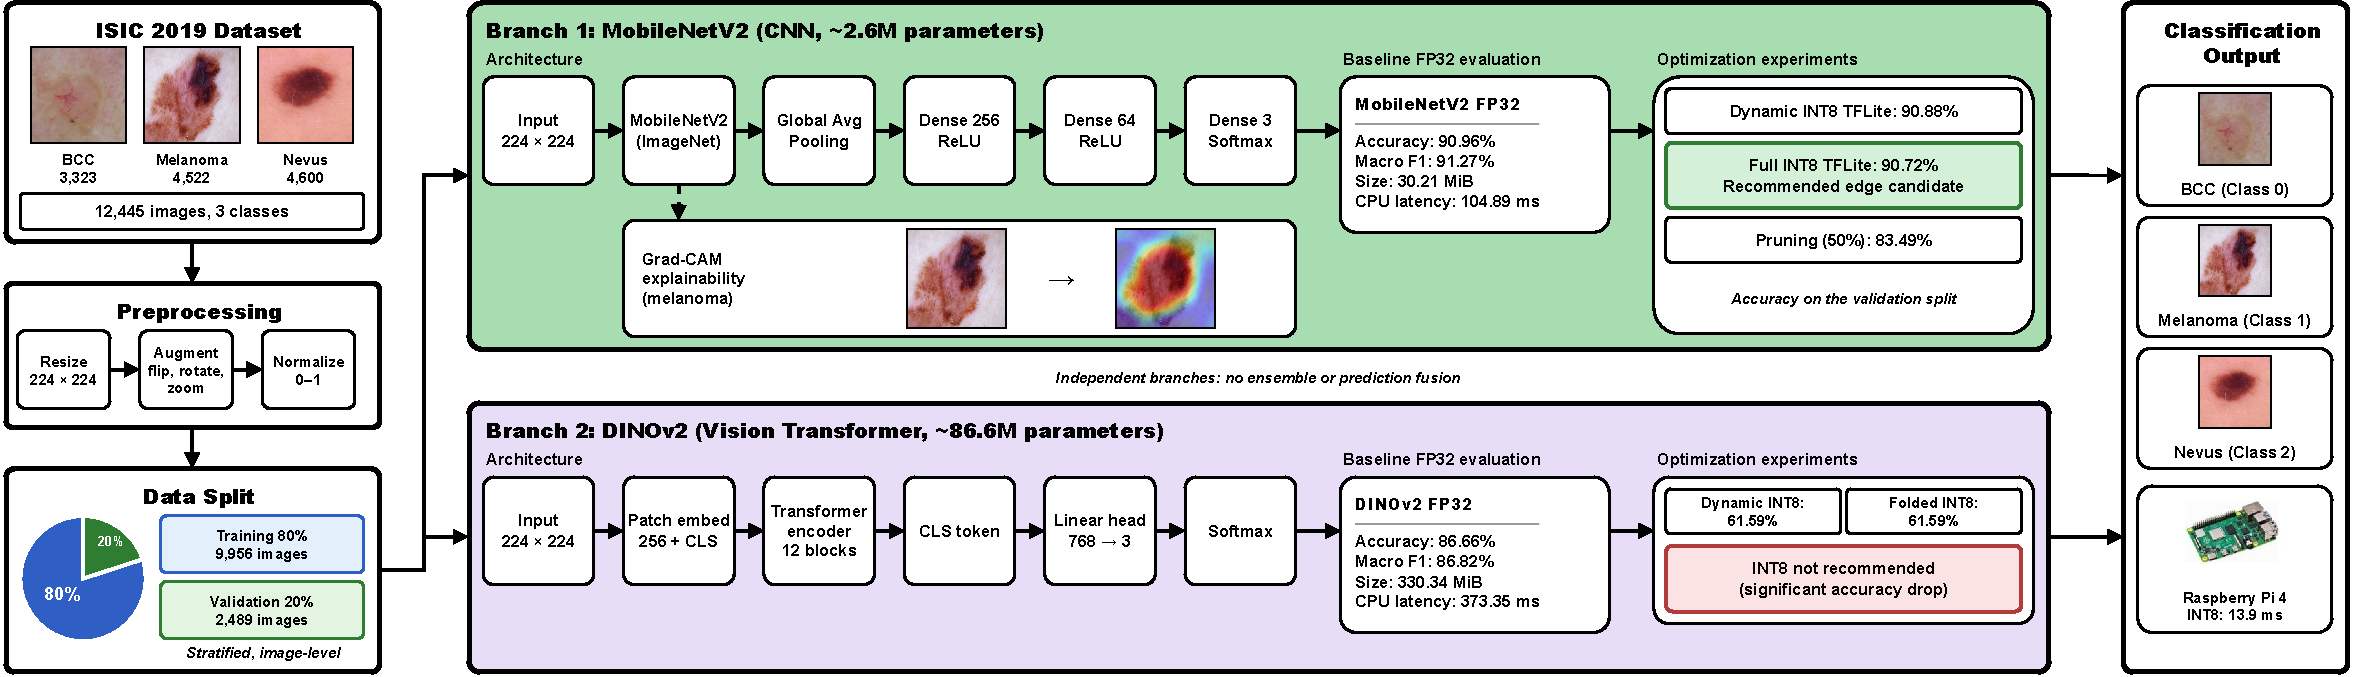
\includegraphics[width=\textwidth]{dermavision_architecture.pdf}
\caption{Overall architecture of the DermaVision framework: data preparation, the MobileNetV2 and DINOv2 branches with their baseline FP32 evaluation and optimization experiments, Grad-CAM explainability, and the three output classes. Accuracy values refer to the 2,489-image validation split.}
\label{fig:architecture}
\end{figure*}

\subsection{Dataset}
\label{sec:dataset}

We used a three-class subset of the ISIC 2019 skin lesion dataset \cite{isic2019kaggle}, which combines images from the HAM10000 \cite{tschandl2018}, BCN20000 \cite{combalia2019}, and ISIC 2017 challenge \cite{codella2018} collections. The three categories considered in this work were Basal Cell Carcinoma (BCC), Melanoma, and Nevus. They cover a malignant melanocytic lesion, its most common benign look-alike, and the most common non-melanocytic skin cancer, which isolates the clinically most consequential Melanoma--Nevus confusion. The subset contains 3,323 BCC, 4,522 Melanoma, and 4,600 Nevus images (largest-to-smallest ratio 1.38), so the classes are close to balanced. Both models used the same label order, so their probability outputs line up with the ground truth.

The class mapping used in this work is shown in Table~\ref{tab:class_mapping}.

\begin{table}[htbp]
\centering
\caption{Class mapping used for skin lesion classification.}
\label{tab:class_mapping}

\begin{tabular*}{\hsize}{@{\extracolsep{\fill}}cc}
\toprule
\textbf{Class Label} & \textbf{Skin Lesion Category} \\
\colrule
0 & BCC \\
1 & Melanoma \\
2 & Nevus \\
\botrule
\end{tabular*}

\end{table}

For final comparative evaluation, an image-level validation partition containing 2,489 images was used: 665 BCC, 904 Melanoma, and 920 Nevus images. The same class-label mapping and image ordering were maintained while generating predictions from MobileNetV2 and DINOv2 so that the predictions of both models could be compared image by image. This partition is not treated as an independent test set.

\subsection{Data Splitting and Leakage Audit}
\label{sec:splitting}

The legacy evaluation protocol used a stratified image-level 80:20 split, producing 9,956 training images and 2,489 validation images. A subsequent lesion-ID audit identified 5,502 unique known lesions and 1,886 images without a lesion ID. Of the validation images, 1,345 (54.04\%) belonged to lesions also represented in the training partition. The overlap was particularly high for BCC (85.11\% of validation images) and Melanoma (79.31\%), while the corresponding Nevus overlap was 6.74\%.

This overlap matters when reading the results. On the clean non-overlapping subset of 1,144 validation images, MobileNetV2 accuracy decreased from 90.96\% to 86.80\%, DINOv2 accuracy decreased from 86.66\% to 84.00\%, and the post-hoc equal-weight fusion decreased from 91.36\% to 87.15\%. We have prepared lesion-grouped splits for retraining. Until those models are trained, the numbers in this paper describe relative model and compression behaviour on the legacy validation partition.

\subsection{Data Preprocessing}
\label{sec:preprocessing}

The input dermoscopic images were resized to $224\times224$ pixels. MobileNetV2 inputs were converted to RGB and scaled by $1/255$ to the range $[0,1]$. DINOv2 inputs were normalized using the ImageNet mean and standard deviation. The verified MobileNetV2 training pipeline used rotation, zoom, and translation augmentation. Horizontal flipping and brightness augmentation are not claimed for the reported run. The images were then converted to tensors and passed to each model.

\subsection{MobileNetV2-Based Classification}
\label{sec:mobilenet}

The CNN branch is an ImageNet-pretrained MobileNetV2 \cite{sandler2018} with a new three-class head for BCC, Melanoma, and Nevus. We trained it for 50 epochs and logged training and validation accuracy and loss after every epoch; these logs give the curves in Fig.~\ref{fig:training_curves}. The recorded epoch history reached 90.12\% validation accuracy at epoch 50; the saved FP32 checkpoint achieved 90.96\% on the consolidated 2,489-image evaluation partition.

\subsection{DINOv2-Based Classification}
\label{sec:dinov2}

The transformer branch is a pretrained DINOv2 encoder with a three-class classification head, trained for 50 epochs with the same per-epoch logging. The recorded epoch history reached 86.82\% validation accuracy at epoch 35; the saved FP32 checkpoint achieved 86.66\% on the consolidated evaluation partition.

\subsection{Post-hoc Fusion Audit}
\label{sec:ensemble}

To test whether the two branches carry complementary information, their probability vectors were combined after training, as defined in Equation~\eqref{eq:ensemble}:

\begin{equation}
P_{\text{fused}} = w_M P_M + w_D P_D, \qquad w_M + w_D = 1, \qquad \hat{y} = \arg\max(P_{\text{fused}})
\label{eq:ensemble}
\end{equation}

Here, $P_M$ and $P_D$ are the probability vectors of MobileNetV2 and DINOv2, and $w_M$ and $w_D$ are their weights. This fusion is an audit only and is not part of the DermaVision pipeline shown in Figure~\ref{fig:architecture}. Its results are reported in Section~\ref{sec:ensembleperf}.

\subsection{System Implementation and Edge Deployment}
\label{sec:implementation}

We packaged the classifier as a Streamlit application. An uploaded dermoscopic image first passes an image quality check; accepted images are preprocessed and classified by the MobileNetV2 TFLite model. The interface then shows the predicted class together with the confidence score for each of BCC, Melanoma, and Nevus. Figure~\ref{fig:workflow} illustrates the implemented application workflow, including the diagnostic interface, image quality assessment stage, and final prediction output.

\begin{figure*}[htbp]
\centering
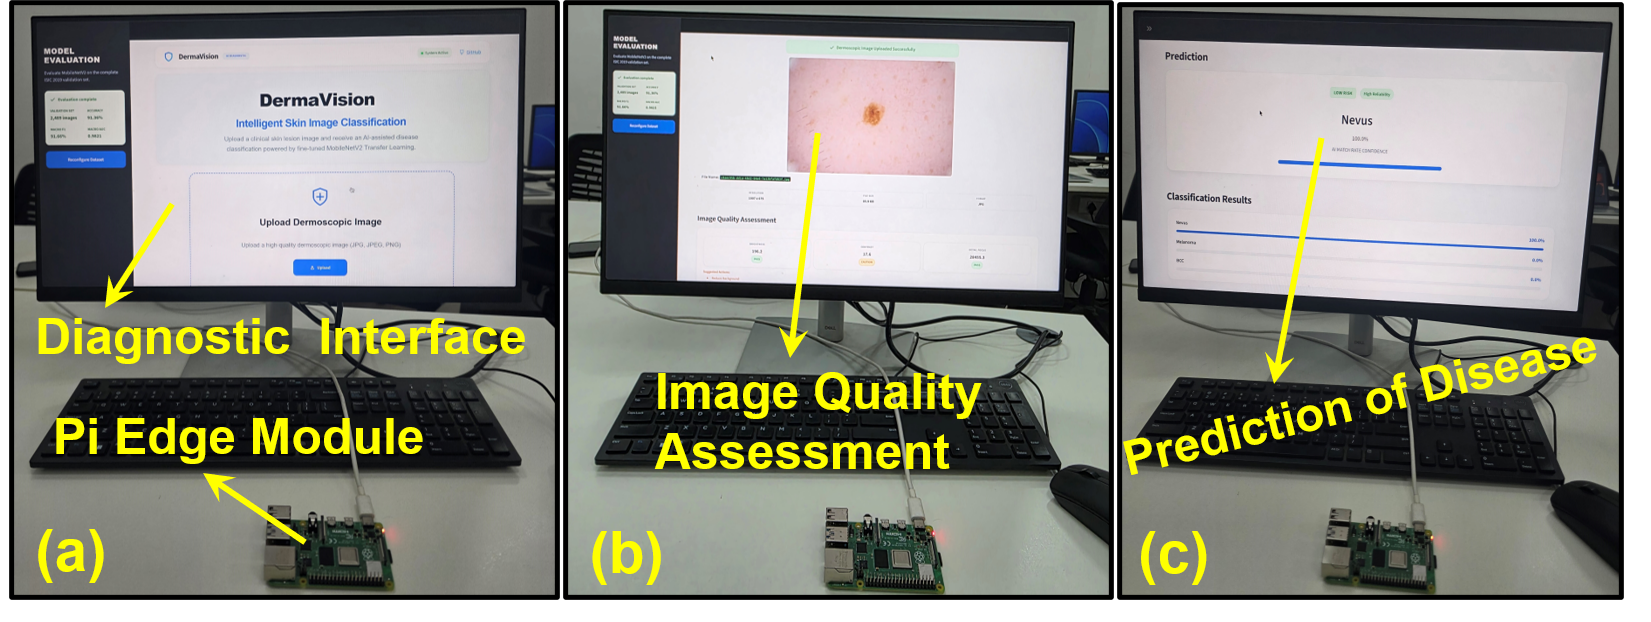
\includegraphics[width=0.82\textwidth]{Picture1-d}
\caption{Application workflow showing (a) the diagnostic interface and Pi Edge Module, (b) the image quality assessment stage, and (c) the final disease prediction with confidence scores.}
\label{fig:workflow}
\end{figure*}

The application currently uses the Dynamic-Range TFLite MobileNetV2 model. A separate Full INT8 TFLite inference module is available and is the recommended edge candidate; its Raspberry Pi 4 latency, memory, and thermal behaviour are reported in Section~\ref{sec:pi}.

% ============================================================
\section{Experimental Results and Analysis}
\label{sec:results}
% ============================================================

\subsection{Experimental Setup}
\label{sec:setup}

Both models were trained for 50 epochs on the three-class subset. The evaluation compared seven variants using accuracy, precision, recall, F1-score, model size, and batch-one host-CPU latency. On-device measurements on a Raspberry Pi 4 are reported separately in Section~\ref{sec:pi}.

\subsection{Individual Model Performance}
\label{sec:individual}

Figure~\ref{fig:training_curves}(a,b) shows how MobileNetV2 trained. Validation accuracy reached 90.12\% at epoch 50, and the saved FP32 checkpoint scored 90.96\% on the consolidated validation partition.

DINOv2 (Fig.~\ref{fig:training_curves}(c,d)) peaked earlier, at 86.82\% validation accuracy in epoch 35, and its saved FP32 checkpoint scored 86.66\% on the same partition.

\begin{figure*}[htbp]
\centering
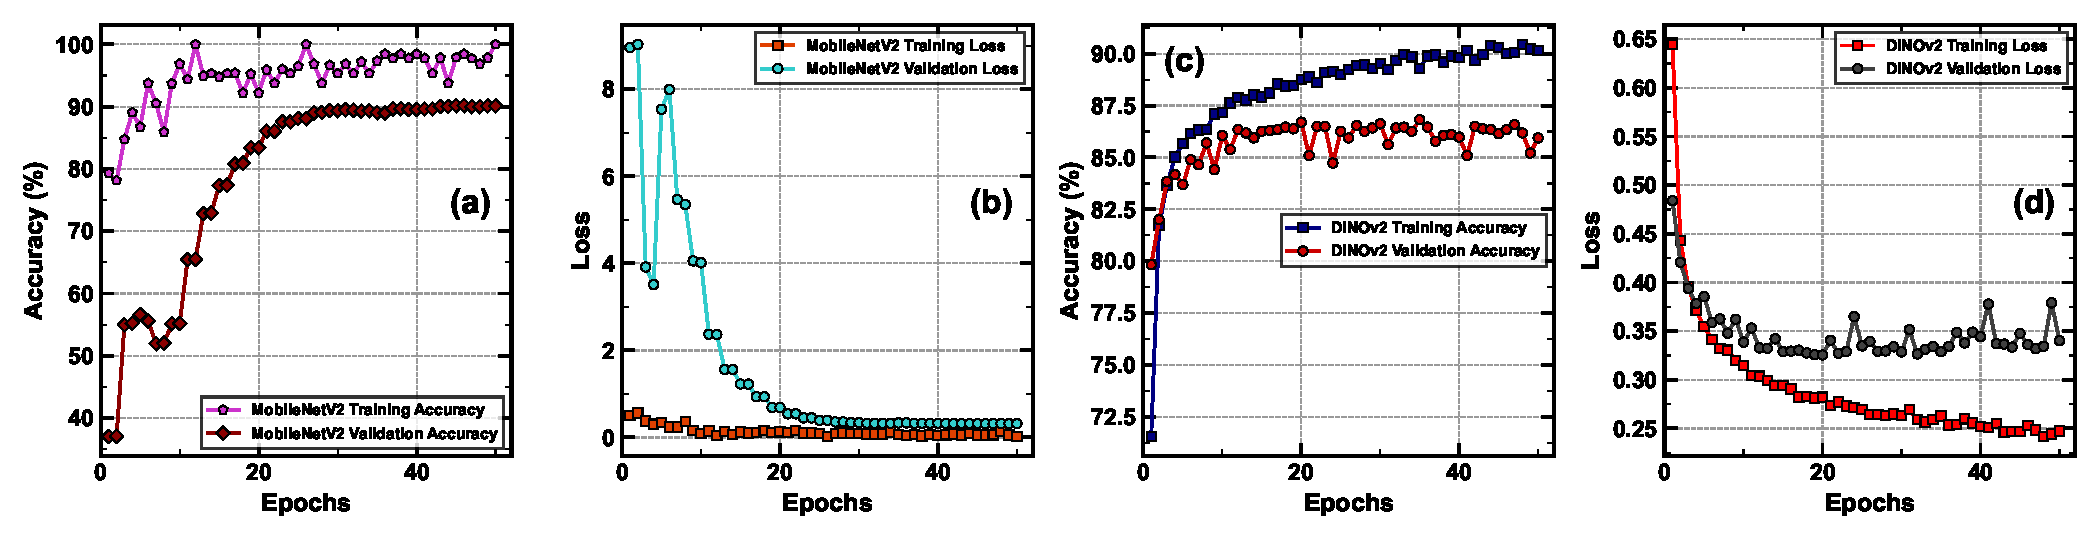
\includegraphics[width=\textwidth]{training_curves.pdf}
\caption{Recorded training and validation curves over 50 epochs: (a) MobileNetV2 accuracy, (b) MobileNetV2 loss, (c) DINOv2 accuracy, and (d) DINOv2 loss. MobileNetV2 reached its highest validation accuracy of 90.16\% at epoch 45 (90.12\% at epoch 50); DINOv2 reached 86.82\% at epoch 35.}
\label{fig:training_curves}
\end{figure*}

\subsection{Comparison of Individual Models}

The consolidated results show that MobileNetV2 FP32 achieved 90.96\% accuracy, 91.27\% Macro F1, and 87.06\% Melanoma recall. DINOv2 FP32 achieved 86.66\% accuracy, 86.82\% Macro F1, and 79.09\% Melanoma recall. These values are validation results from the image-level partition described in Section~\ref{sec:splitting}.

Because MobileNetV2 achieved the higher accuracy at a fraction of the size and latency of DINOv2, it is treated as the primary deployment branch, while DINOv2 is retained as the transformer comparison branch.

\subsection{Post-hoc Fusion Audit Results}
\label{sec:ensembleperf}

Table~\ref{tab:ensemble_results} compares MobileNetV2 with the two audited fusion configurations. The previously reported configuration ($w_M=0.4$, $w_D=0.6$) achieved 90.76\% accuracy and 85.18\% Melanoma recall, both below MobileNetV2 alone. The equal-weight configuration ($w_M=0.5$, $w_D=0.5$) exceeded MobileNetV2 by only 0.40 percentage points, with weights evaluated on the same validation predictions and on a partition with documented lesion overlap. Because this gain is small, unverified on held-out data, and requires running the 330.34 MiB DINOv2 model alongside MobileNetV2, fusion is not adopted, and the remaining analysis focuses on the independent branches.

The two branches make partly different errors: DINOv2 correctly classified 110 images that MobileNetV2 misclassified, but misclassified 217 images that MobileNetV2 classified correctly. Equal-weight fusion corrected 27 MobileNetV2 errors and introduced 17 new ones, a net gain of 10 images, and raised recall in every class (BCC $+0.30$, Melanoma $+0.33$, Nevus $+0.54$ percentage points). An exact two-sided McNemar test on these discordant pairs gave $p = 0.174$, so the improvement is not statistically significant at the 0.05 level; the test also assumes independent samples, which the documented lesion overlap only partly satisfies. On the 1,144 non-overlapping validation images the gain was 0.35 percentage points (87.15\% versus 86.80\%).

\begin{table}[htbp]
\centering
\caption{Post-hoc fusion audit compared with MobileNetV2 alone on the validation partition.}
\label{tab:ensemble_results}

\begin{tabular*}{\hsize}{@{\extracolsep{\fill}}lccc}
\toprule
\textbf{Model / Configuration} & \textbf{Accuracy} & \textbf{Macro F1} & \textbf{Melanoma Recall} \\
\colrule
MobileNetV2 FP32 (adopted) & 90.96\% & 91.27\% & 87.06\% \\
Fusion audit ($w_M=0.5$, $w_D=0.5$) & 91.36\% & 91.67\% & 87.39\% \\
Fusion audit ($w_M=0.4$, $w_D=0.6$) & 90.76\% & 91.01\% & 85.18\% \\
\botrule
\end{tabular*}

\end{table}

\subsection{Compression and Development-CPU Deployment Analysis}
\label{sec:compression}

Table~\ref{tab:compression_results} summarizes the principal compression and deployment measurements. Full INT8 TFLite MobileNetV2 reduced storage by 90.27\% relative to the FP32 checkpoint and retained accuracy within 0.24 percentage points. It also achieved 4.51 ms batch-one latency on the benchmark host. In contrast, 50\% unstructured magnitude pruning \cite{han2015} reduced accuracy by 7.47 percentage points and Melanoma recall by 13.61 percentage points without providing a dense CPU speedup. DINOv2 FP32 required 330.34 MiB on disk and showed 235.09--373.35 ms host latency. Native dynamic INT8 reduced DINOv2 storage to 87.38 MiB and latency to 173.54 ms, which gives a baseline of 61.59\% accuracy and 49.67\% Melanoma recall for later quantization-aware work.

\begin{table}[htbp]
\centering
\caption{Consolidated validation and development-CPU deployment measurements.}
\label{tab:compression_results}
\begin{tabular*}{\hsize}{@{\extracolsep{\fill}}lcccc}
\toprule
\textbf{Model} & \textbf{Accuracy} & \textbf{Macro F1} & \textbf{Mel. Recall} & \textbf{Size / Latency} \\
\colrule
MobileNetV2 FP32 & 90.96\% & 91.27\% & 87.06\% & 30.21 MiB / 104.89 ms \\
MobileNetV2 Dynamic TFLite & 90.88\% & 91.20\% & 85.62\% & 2.74 MiB / 27.76 ms \\
MobileNetV2 Full INT8 TFLite & \textbf{90.72\%} & \textbf{91.03\%} & \textbf{86.73\%} & \textbf{2.94 MiB / 4.51 ms} \\
MobileNetV2 50\% Pruned & 83.49\% & 83.55\% & 73.45\% & 30.21 MiB / 101.54 ms \\
DINOv2 FP32 & 86.66\% & 86.82\% & 79.09\% & 330.34 MiB / 235--373 ms \\
DINOv2 Dynamic INT8 & 61.59\% & 57.54\% & 49.67\% & 87.38 MiB / 173.54 ms \\
\botrule
\end{tabular*}
\end{table}

The DINOv2 INT8 drop has a clear cause. Layer-wise diagnostics identified extreme activation outliers in transformer Blocks 8--11, a known obstacle to post-training transformer quantization \cite{bondarenko2021,dettmers2022}, with magnitudes up to approximately 494.72 compared with upper-percentile values near 1.3--2.7 in the corresponding diagnostic summaries. Handling these outliers, through quantization-aware training, per-channel scaling, better calibration, or distillation to ViT-S, is the main task before DINOv2 can be deployed.

\subsection{Raspberry Pi 4 On-Device Benchmark}
\label{sec:pi}

All MobileNetV2 variants were benchmarked on a Raspberry Pi 4 Model B (Broadcom BCM2711, four Cortex-A72 cores at up to 1.8\,GHz, 4\,GB RAM, 64-bit Raspberry Pi OS, Python 3.13.5) without any hardware accelerator. TFLite models were executed with ai-edge-litert 2.3.0 (XNNPACK, four threads) and the FP32 Keras model with TensorFlow 2.21.0 \cite{abadi2016}, using the same batch-one protocol as on the development CPU (50 warm-up and 200 timed runs on a preloaded tensor). The model files were byte-identical to those evaluated on the development CPU, so the accuracy values in Table~\ref{tab:compression_results} apply unchanged; every variant predicted the same class for the benchmark image. An unquantized FP32 TFLite conversion was also measured to separate the effect of the runtime from that of quantization. Table~\ref{tab:pi_results} summarizes the results.

\begin{table}[htbp]
\centering
\caption{Raspberry Pi 4 Model B results for MobileNetV2 (batch one, four threads). Peak RSS is the memory of the whole Python process; Max temp.\ is the peak SoC temperature during a 300\,s continuous run.}
\label{tab:pi_results}
\begin{tabular*}{\hsize}{@{\extracolsep{\fill}}lccccc}
\toprule
\textbf{Variant} & \textbf{Disk} & \textbf{Latency (ms)} & \textbf{FPS} & \textbf{Peak RSS} & \textbf{Max temp.} \\
\colrule
FP32 Keras & 30.21 MiB & 597.59 $\pm$ 9.86 & 1.67 & 636.9 MiB & 55.0\,$^\circ$C \\
FP32 TFLite (unquantized) & 9.79 MiB & 36.63 $\pm$ 0.34 & 27.30 & 69.5 MiB & 74.5\,$^\circ$C \\
Dynamic-range INT8 TFLite & 2.74 MiB & 41.72 $\pm$ 3.42 & 23.97 & 59.2 MiB & 72.0\,$^\circ$C \\
\textbf{Full INT8 TFLite} & \textbf{2.94 MiB} & \textbf{13.92 $\pm$ 0.20} & \textbf{71.83} & \textbf{51.7 MiB} & \textbf{78.4\,$^\circ$C} \\
\botrule
\end{tabular*}
\end{table}

Full INT8 TFLite ran at 13.92 ms per image (71.8 FPS), 42.9$\times$ faster than FP32 Keras and 2.6$\times$ faster than unquantized FP32 TFLite, while using the least memory. Most of the FP32 Keras latency is runtime overhead: converting the same FP32 weights to TFLite reduced latency from 597.59 ms to 36.63 ms. Dynamic-range quantization reduced storage to 2.74 MiB but was slightly slower than FP32 TFLite (41.72 ms), because its weights are dequantized during inference \cite{krishnamoorthi2018}; only full-integer quantization delivered a speedup on the Cortex-A72. With a single thread, Full INT8 required 45.86 ms and Dynamic-range 65.11 ms. Including decoding and preprocessing of a $1024 \times 1024$ PNG input, the Full INT8 end-to-end latency was 106.08 ms, so image decoding rather than inference dominates the on-device pipeline.

Sustained behaviour was measured by running each variant continuously for 300\,s from a starting temperature below 50\,$^\circ$C, while sampling the SoC temperature, ARM clock, and firmware throttling flags every 2\,s. No throttling or under-voltage flag was raised in any run. Full INT8, which kept all four cores busy and completed 21,118 inferences, reached the highest temperature (78.4\,$^\circ$C), yet its mean latency was unchanged between the first and last 10\% of the run (14.11 and 14.16\,ms). FP32 Keras reached only 55.0\,$^\circ$C because it did not saturate the CPU.

\subsection{Confusion Matrix and Error Analysis}
\label{sec:erroranalysis}

Figure~\ref{fig:confusion_matrix} presents the confusion matrix of MobileNetV2 FP32 for the three target classes: BCC, Melanoma, and Nevus. The diagonal elements represent correctly classified samples, while the off-diagonal elements represent misclassifications.

\begin{figure}[htbp]
\centering
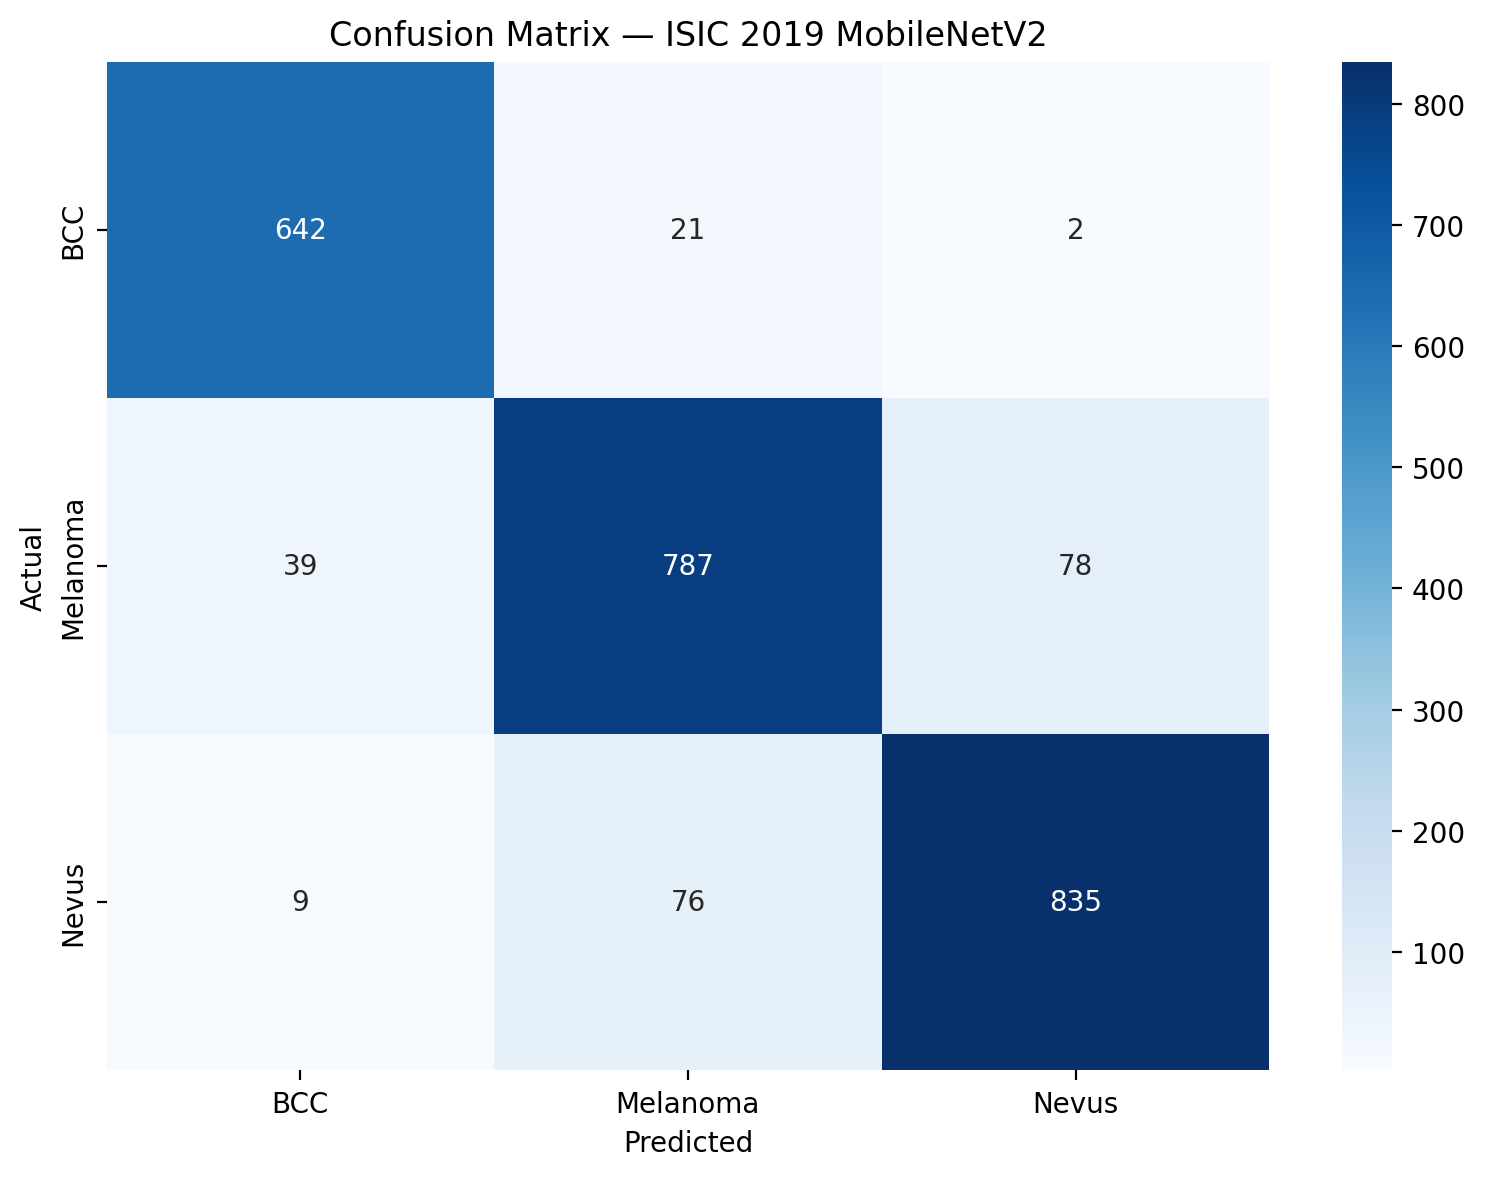
\includegraphics[width=0.36\textwidth]{mobilenetv2_confusion_matrix.png}
\caption{Confusion matrix of MobileNetV2 FP32 for BCC, Melanoma, and Nevus classification on the 2,489-image validation partition.}
\label{fig:confusion_matrix}
\end{figure}

For the BCC class, 642 images were correctly classified, 21 were predicted as Melanoma, and 2 were predicted as Nevus. For the Melanoma class, 787 images were correctly classified, 39 were predicted as BCC, and 78 were predicted as Nevus. For the Nevus class, 835 images were correctly classified, 9 were predicted as BCC, and 76 were predicted as Melanoma.

Table~\ref{tab:perclass} presents the class-level precision, recall, and F1-score values derived from the confusion matrix.

\begin{table}[htbp]
\centering
\caption{Class-level performance of MobileNetV2 FP32.}
\label{tab:perclass}

\begin{tabular*}{\hsize}{@{\extracolsep{\fill}}lcccc}
\toprule
\textbf{Class} & \textbf{Support} & \textbf{Precision} & \textbf{Recall} & \textbf{F1-score} \\
\colrule
BCC       & 665 & 93.04\% & 96.54\% & 94.76\% \\
Melanoma  & 904 & 89.03\% & 87.06\% & 88.03\% \\
Nevus     & 920 & 91.26\% & 90.76\% & 91.01\% \\
\colrule
Macro avg & 2,489 & 91.11\% & 91.45\% & 91.27\% \\
\botrule
\end{tabular*}

\end{table}

BCC achieved the highest recall, while Melanoma achieved the lowest. The confusion between Melanoma and Nevus is the main source of classification error: 78 Melanoma images were predicted as Nevus, and 76 Nevus images were predicted as Melanoma.

% ============================================================
\section{Discussion}
\label{sec:discussion}
% ============================================================

MobileNetV2 gives the best balance of accuracy and cost among the variants we tested. Its FP32 checkpoint achieved 90.96\% validation accuracy and 87.06\% Melanoma recall, while Full INT8 conversion retained 90.72\% accuracy and 86.73\% Melanoma recall with a substantially smaller model and lower host-CPU latency. On a Raspberry Pi 4 it ran at 71.8 FPS, which confirms Full INT8 MobileNetV2 as a practical edge model.

Fusion helped only a little. The 0.4/0.6 weighting (90.76\%) stayed below MobileNetV2, and equal weighting added 0.40 percentage points, with weights chosen on the same validation predictions. The equal-weight fusion was also 7.79 percentage points less accurate on clean than on overlapping validation images. That gain does not justify running DINOv2 next to MobileNetV2 on an edge device, so the branches stay separate.

Melanoma remains the hardest class, mostly because of its confusion with Nevus. Pruning made this worse: at 50\% sparsity and without a sparse execution engine, Melanoma recall fell by 13.61 percentage points. For DINOv2, the INT8 results point to activation calibration as the main obstacle to compressing the transformer.

The Streamlit application still runs the Dynamic-Range TFLite model rather than the Full INT8 one. Apart from the McNemar test of the fusion audit, no confidence intervals, skin-tone fairness evaluation, or lesion-disjoint retrained test result are available in the present study. The dataset also contains only three of the eight ISIC 2019 categories, includes 1,886 images without lesion IDs, and has no external multi-centre validation. For these reasons, the results should not be read as clinical evidence.

% ============================================================
\section{Grad-CAM Explainability}
\label{sec:prediction_results}

Figure~\ref{fig:gradcam} shows Grad-CAM \cite{selvaraju2017} heatmaps computed on the final convolutional layer of MobileNetV2 ($7 \times 7 \times 1280$) for one correctly classified image of each class and for a Melanoma image predicted as Nevus. In the correct cases, the activation is concentrated on the lesion rather than on the surrounding skin, hair, or imaging artefacts. In the failure case, the model also attends to the lesion but still predicts Nevus, which indicates that the error arises from how the lesion is interpreted rather than from attention to irrelevant regions. Grad-CAM is a coarse post-hoc attribution and does not establish clinical explainability.

\begin{figure}[htbp]
\centering
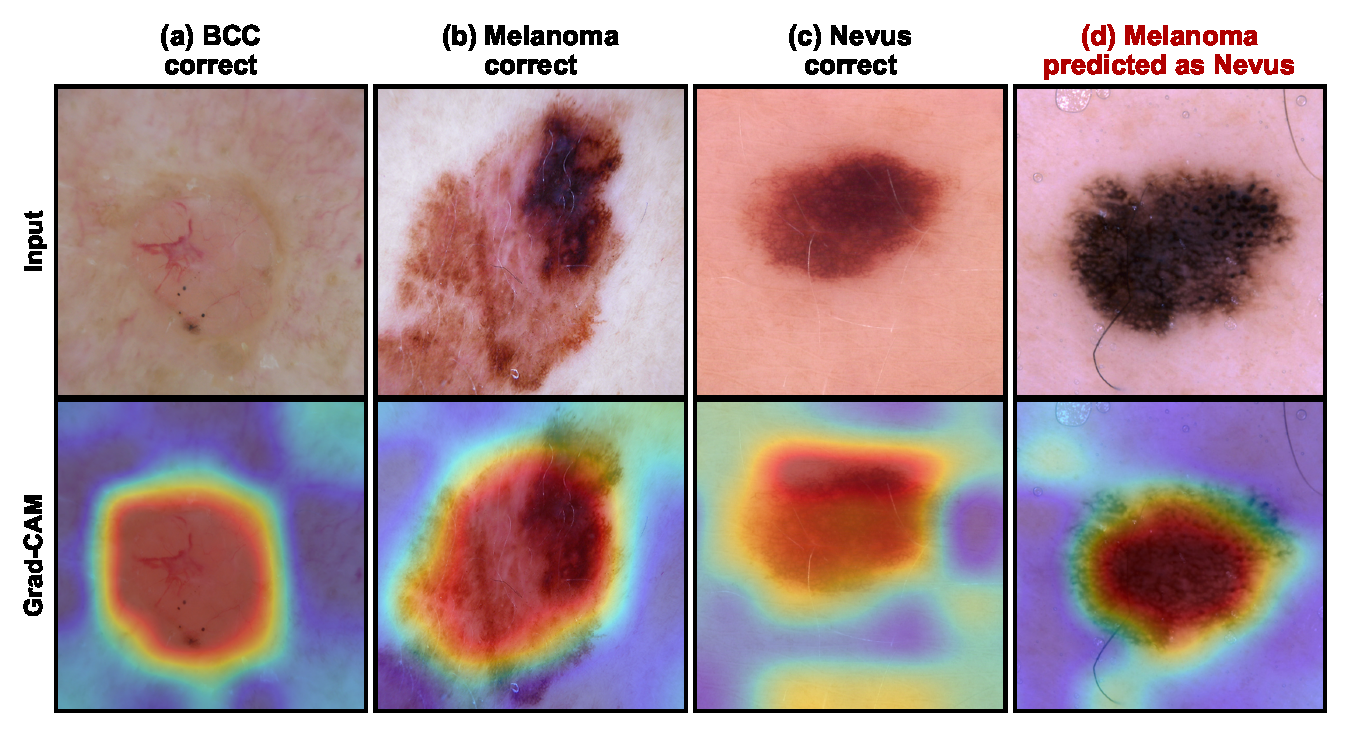
\includegraphics[width=0.62\textwidth]{gradcam_figure.pdf}
\caption{Grad-CAM heatmaps of MobileNetV2 FP32: (a)--(c) correctly classified BCC, Melanoma, and Nevus images; (d) a Melanoma image predicted as Nevus. Top: input; bottom: heatmap overlay.}
\label{fig:gradcam}
\end{figure}
\section{Conclusion and Future Work}
\label{sec:conclusion}
% ============================================================

This work presented a comparative study of MobileNetV2 and DINOv2 for three-class skin lesion classification. On the legacy image-level validation partition, MobileNetV2 FP32 achieved 90.96\% accuracy, while Full INT8 TFLite reduced storage to 2.94 MiB and retained 90.72\% accuracy with 86.73\% Melanoma recall. Fusing the two models added 0.40 percentage points, which was not statistically significant (McNemar $p = 0.174$), so the branches are kept independent. Because the validation partition shares 54.04\% of its lesions with training, these are not independent test results. Full INT8 MobileNetV2 is the current edge baseline, and the DINOv2 experiments show that activation calibration is what its compression needs.

In practice, Full INT8 MobileNetV2 is ready for edge testing now, and the DINOv2 INT8 result gives a measured starting point for quantization-aware redesign and distillation. On a Raspberry Pi 4 it reached 13.92 ms per image (71.8 FPS) with 51.7 MiB peak memory, compared with 597.59 ms for FP32 Keras.

Future work will retrain both branches using the prepared zero-overlap lesion-grouped split, freeze any Melanoma safety threshold on validation data, re-test fusion on the lesion-disjoint split, and perform one final held-out test evaluation. Further work should include paired statistical tests, confidence intervals, power measurements and testing on additional edge devices, attention rollout for DINOv2, skin-tone fairness analysis, calibration, and comparison with external datasets. Extending the study to all eight ISIC 2019 categories, quantization-aware training, ViT-S distillation, out-of-distribution rejection, and imbalance-aware losses may improve the reliability of a future deployment-oriented system.

% ============================================================
\section*{Acknowledgment}

The authors would like to thank Amrita Vishwa Vidyapeetham, Chennai Campus, for providing the computing infrastructure and academic support for this work. The authors also acknowledge the AI DISC Lab and the NEGCES Lab for their support and facilities during the development and evaluation of this work.
\begin{thebibliography}{99}
% ============================================================

\bibitem{sandler2018}
Sandler, Mark, Andrew Howard, Menglong Zhu, Andrey Zhmoginov, and Liang-Chieh Chen. (2018) ``MobileNetV2: Inverted residuals and linear bottlenecks.'' {\it Proceedings of the IEEE Conference on Computer Vision and Pattern Recognition}: 4510--4520.

\bibitem{oquab2024}
Oquab, Maxime, Timoth\'{e}e Darcet, Th\'{e}o Moutakanni, Huy Vo, Marc Szafraniec, Vasil Khalidov, Pierre Fernandez, et al. (2024) ``DINOv2: Learning robust visual features without supervision.'' {\it Transactions on Machine Learning Research}.

\bibitem{esteva2017}
Esteva, Andre, Brett Kuprel, Roberto A. Novoa, Justin Ko, Susan M. Swetter, Helen M. Blau, and Sebastian Thrun. (2017) ``Dermatologist-level classification of skin cancer with deep neural networks.'' {\it Nature} {\bf 542} (7639): 115--118.

\bibitem{he2016}
He, Kaiming, Xiangyu Zhang, Shaoqing Ren, and Jian Sun. (2016) ``Deep residual learning for image recognition.'' {\it Proceedings of the IEEE Conference on Computer Vision and Pattern Recognition}: 770--778.

\bibitem{howard2017}
Howard, Andrew G., Menglong Zhu, Bo Chen, Dmitry Kalenichenko, Weijun Wang, Tobias Weyand, Marco Andreetto, and Hartwig Adam. (2017) ``MobileNets: Efficient convolutional neural networks for mobile vision applications.'' {\it arXiv preprint} arXiv:1704.04861.

\bibitem{dosovitskiy2021}
Dosovitskiy, Alexey, Lucas Beyer, Alexander Kolesnikov, Dirk Weissenborn, Xiaohua Zhai, Thomas Unterthiner, Mostafa Dehghani, et al. (2021) ``An image is worth 16x16 words: Transformers for image recognition at scale.'' {\it International Conference on Learning Representations}.

\bibitem{caron2021}
Caron, Mathilde, Hugo Touvron, Ishan Misra, Herv\'{e} J\'{e}gou, Julien Mairal, Piotr Bojanowski, and Armand Joulin. (2021) ``Emerging properties in self-supervised vision transformers.'' {\it Proceedings of the IEEE/CVF International Conference on Computer Vision}: 9650--9660.

\bibitem{kittler1998}
Kittler, Josef, Mohamad Hatef, Robert P. W. Duin, and Jiri Matas. (1998) ``On combining classifiers.'' {\it IEEE Transactions on Pattern Analysis and Machine Intelligence} {\bf 20} (3): 226--239.

\bibitem{dietterich2000}
Dietterich, Thomas G. (2000) ``Ensemble methods in machine learning.'' {\it Multiple Classifier Systems, Lecture Notes in Computer Science} {\bf 1857}: 1--15.

\bibitem{deng2009}
Deng, Jia, Wei Dong, Richard Socher, Li-Jia Li, Kai Li, and Li Fei-Fei. (2009) ``ImageNet: A large-scale hierarchical image database.'' {\it Proceedings of the IEEE Conference on Computer Vision and Pattern Recognition}: 248--255.

\bibitem{jacob2018}
Jacob, Benoit, Skirmantas Kligys, Bo Chen, Menglong Zhu, Matthew Tang, Andrew Howard, Hartwig Adam, and Dmitry Kalenichenko. (2018) ``Quantization and training of neural networks for efficient integer-arithmetic-only inference.'' {\it Proceedings of the IEEE Conference on Computer Vision and Pattern Recognition}: 2704--2713.

\bibitem{selvaraju2017}
Selvaraju, Ramprasaath R., Michael Cogswell, Abhishek Das, Ramakrishna Vedantam, Devi Parikh, and Dhruv Batra. (2017) ``Grad-CAM: Visual explanations from deep networks via gradient-based localization.'' {\it Proceedings of the IEEE International Conference on Computer Vision}: 618--626.

\bibitem{isic2019kaggle}
Larxel, ``Skin Lesion Images for Melanoma Classification,'' Kaggle Dataset, 2020. Available: \url{https://www.kaggle.com/datasets/andrewmvd/isic-2019}.

\bibitem{tschandl2018}
Tschandl, Philipp, Cliff Rosendahl, and Harald Kittler. (2018) ``The HAM10000 dataset, a large collection of multi-source dermatoscopic images of common pigmented skin lesions.'' {\it Scientific Data} {\bf 5}: 180161.

\bibitem{combalia2019}
Combalia, Marc, Noel C. F. Codella, Veronica Rotemberg, Brian Helba, Veronica Vilaplana, Ofer Reiter, Cristina Carrera, et al. (2019) ``BCN20000: Dermoscopic lesions in the wild.'' {\it arXiv preprint} arXiv:1908.02288.

\bibitem{codella2018}
Codella, Noel C. F., David Gutman, M. Emre Celebi, Brian Helba, Michael A. Marchetti, Stephen W. Dusza, Aadi Kalloo, et al. (2018) ``Skin lesion analysis toward melanoma detection: A challenge at the 2017 International Symposium on Biomedical Imaging (ISBI), hosted by the International Skin Imaging Collaboration (ISIC).'' {\it IEEE 15th International Symposium on Biomedical Imaging}: 168--172.

\bibitem{han2015}
Han, Song, Jeff Pool, John Tran, and William J. Dally. (2015) ``Learning both weights and connections for efficient neural networks.'' {\it Advances in Neural Information Processing Systems} {\bf 28}: 1135--1143.

\bibitem{bondarenko2021}
Bondarenko, Yelysei, Markus Nagel, and Tijmen Blankevoort. (2021) ``Understanding and overcoming the challenges of efficient transformer quantization.'' {\it Proceedings of the Conference on Empirical Methods in Natural Language Processing}: 7947--7969.

\bibitem{dettmers2022}
Dettmers, Tim, Mike Lewis, Younes Belkada, and Luke Zettlemoyer. (2022) ``LLM.int8(): 8-bit matrix multiplication for transformers at scale.'' {\it Advances in Neural Information Processing Systems} {\bf 35}: 30318--30332.

\bibitem{abadi2016}
Abadi, Mart\'{i}n, Paul Barham, Jianmin Chen, Zhifeng Chen, Andy Davis, Jeffrey Dean, Matthieu Devin, et al. (2016) ``TensorFlow: A system for large-scale machine learning.'' {\it 12th USENIX Symposium on Operating Systems Design and Implementation}: 265--283.

\bibitem{krishnamoorthi2018}
Krishnamoorthi, Raghuraman. (2018) ``Quantizing deep convolutional networks for efficient inference: A whitepaper.'' {\it arXiv preprint} arXiv:1806.08342.

\end{thebibliography}

\end{document}